\chapter{Test of effect run time}\label{app:effect_run_time}

The tests of the time for running each effect are presented in this appendix.

\section*{Materials and setup}
To measure the time consumption of each effect, the following materials are used:
\begin{itemize}
\item Digilent Analog Discovery 2 (Oscilloscope)
\item Digilent Waveforms 2015 (PC - software)
\item TMS320C5515 eZdsp development board
\end{itemize}


\begin{figure}[htbp!]
	\centering
		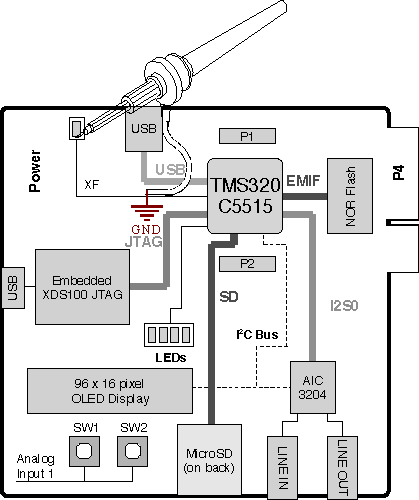
\includegraphics[width=0.5\textwidth]{run_time.pdf}
		\caption{Illustration showing the location of the measurement point on the EZdsp}
		\label{fig:run_time_test_point}
\end{figure}

\includeCode{mainas.asm}{assembly}{12}{21}{Example of runtime testing main program}{code:mainas_asm}{code/design/}

\section*{Test procedure}
\begin{enumerate}
\item The materials are set up as in \autoref{fig:run_time_test_point}.
\item The Digilent Waveform 2015 is set as a Scope.
\item  The XF led bit is set at the beginning of the program and cleared in the end of the program, in the mainas file, see example \autoref{code:mainas_asm}. The time from when the LED is being illuminated until it is turned off is the runtime, also measured using the magnitude as shown in \autoref{fig:run_time_test_point}. 
\item  The oscilloscope is then used to measure the XF LED runtime 
\item The data is plotted in MATLAB.
\end{enumerate}

\section*{Reverb run time}
The following \autoref{fig:reverb_time_test} shows the measurement results of the \gls{reverb} assembly program runtime.
\begin{figure}[htbp!]
	\centering
		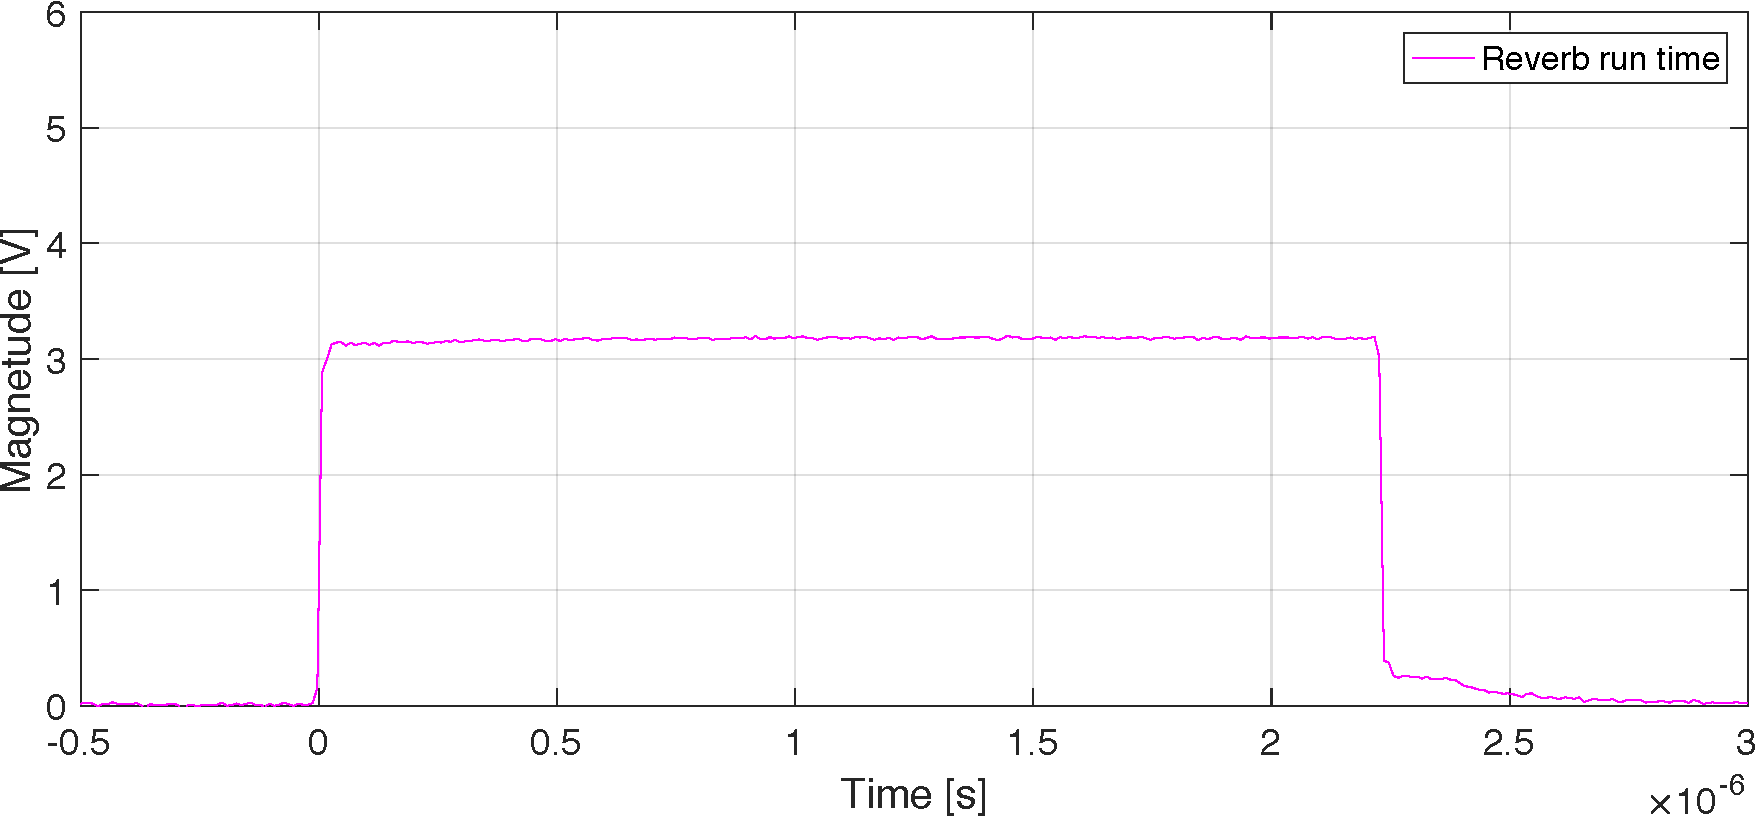
\includegraphics[width=1\textwidth]{reverb_run_time.pdf}
		\caption{The figure shows the runtime of the \gls{reverb} assembly program}
		\label{fig:reverb_time_test}
\end{figure}

According to \autoref{fig:reverb_time_test}, the \gls{reverb} runtime is \SI{2.25}{\micro\second}.

\section*{Cordic run time}
The following \autoref{fig:cordic_time_test} shows the measurement results of the cordic assembly program runtime.
\begin{figure}[htbp!]
	\centering
		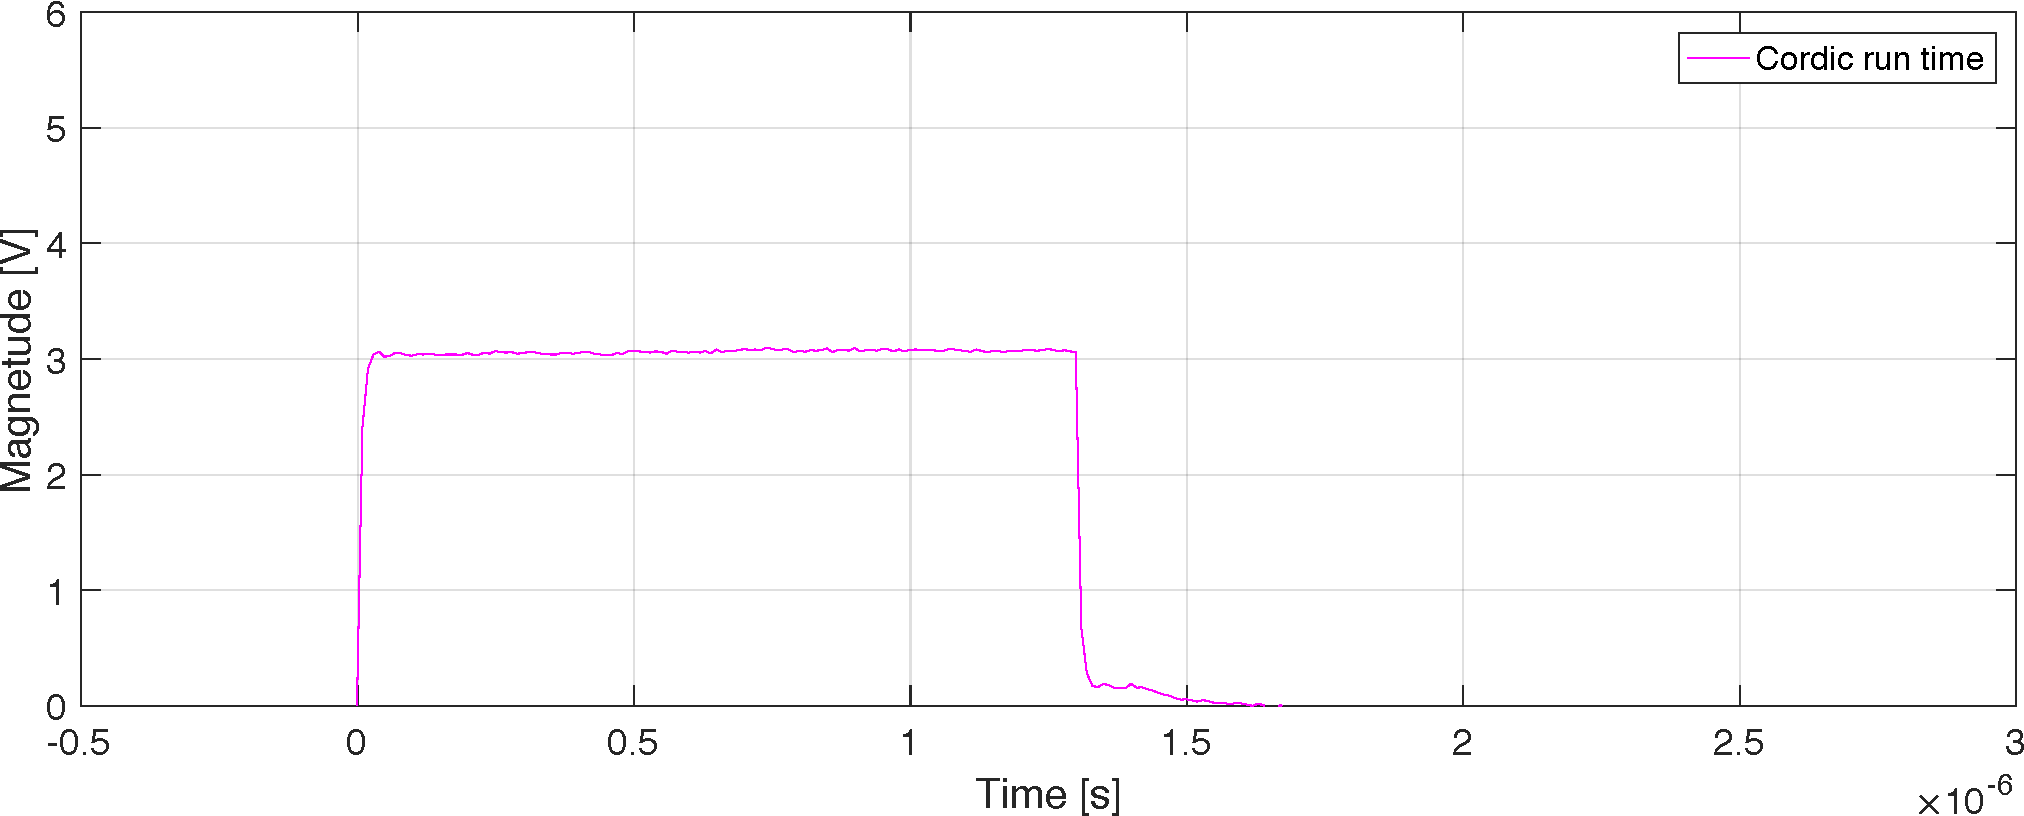
\includegraphics[width=1\textwidth]{cordic_run_time.pdf}
		\caption{The figure shows the runtime of the cordic assembly program}
		\label{fig:cordic_time_test}
\end{figure}

According to \autoref{fig:cordic_time_test}, the cordic runtime is \SI{1.3}{\micro\second}.

\section*{Flanger run time}
The following \autoref{fig:flanger_time_test} shows the measurement results of the flanger assembly program runtime.
\begin{figure}[htbp!]
	\centering
		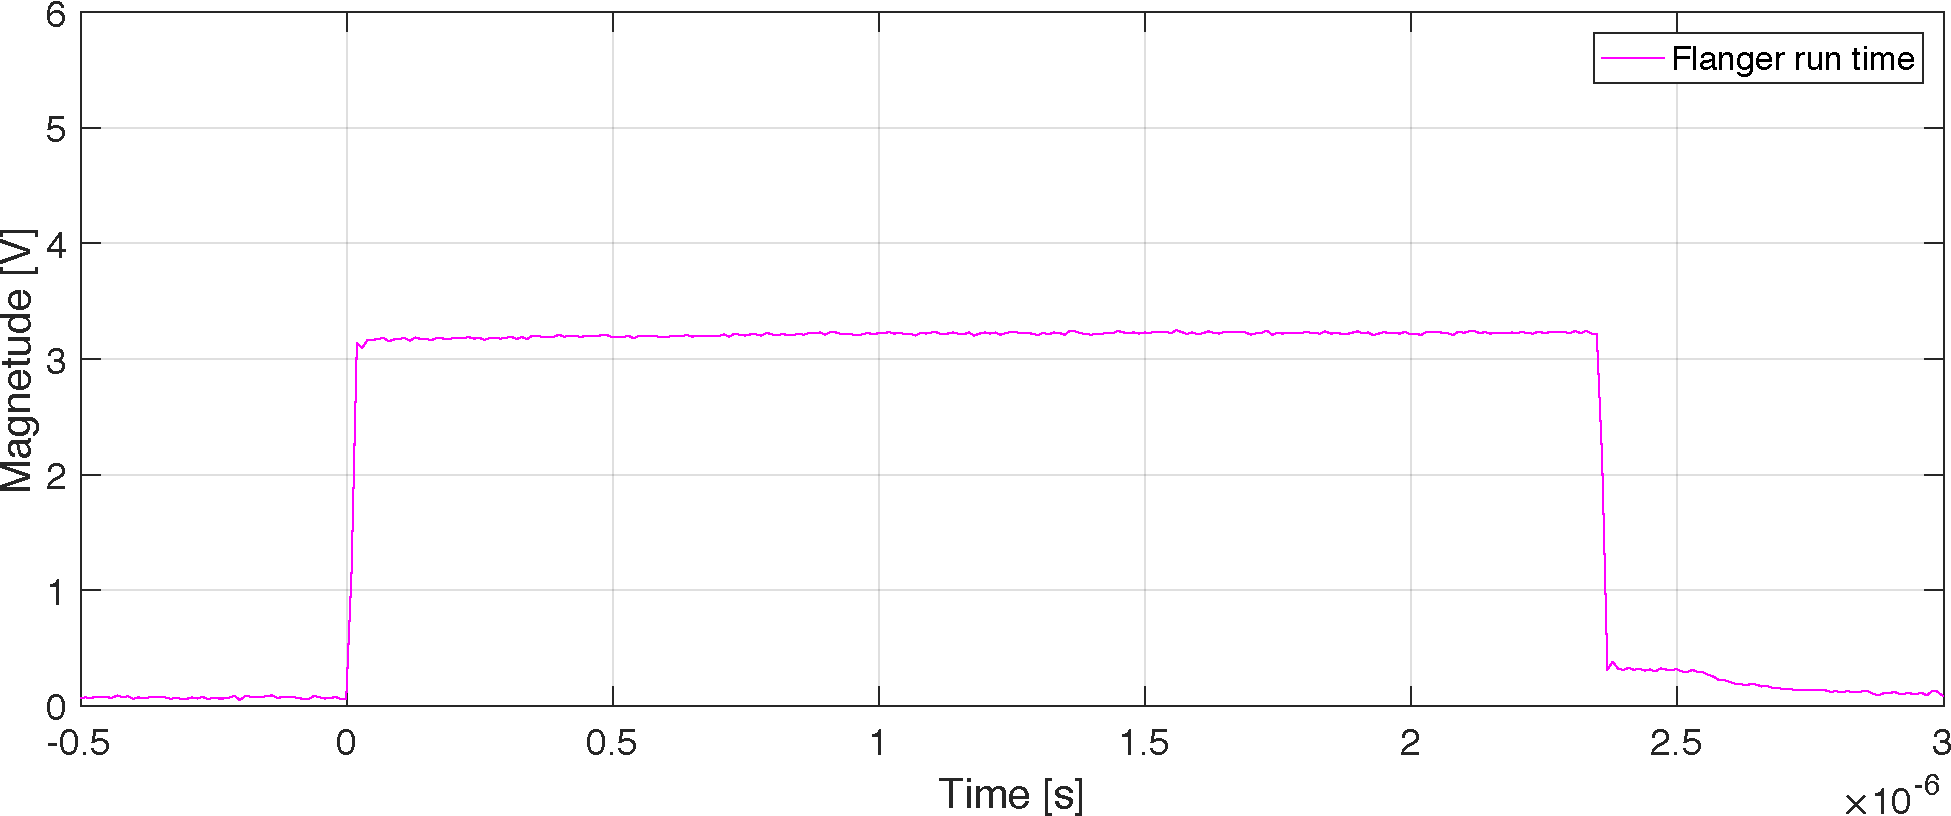
\includegraphics[width=1\textwidth]{flanger_run_time.pdf}
		\caption{The figure shows the runtime of the flanger assembly program}
		\label{fig:flanger_time_test}
\end{figure}

According to \autoref{fig:flanger_time_test}, the flanger run time is \SI{2.25}{\micro\second}.

\section*{EQ run time}
The following \autoref{fig:eq_time_test} shows the measurement results of the flanger assembly program runtime.
\begin{figure}[htbp!]
	\centering
		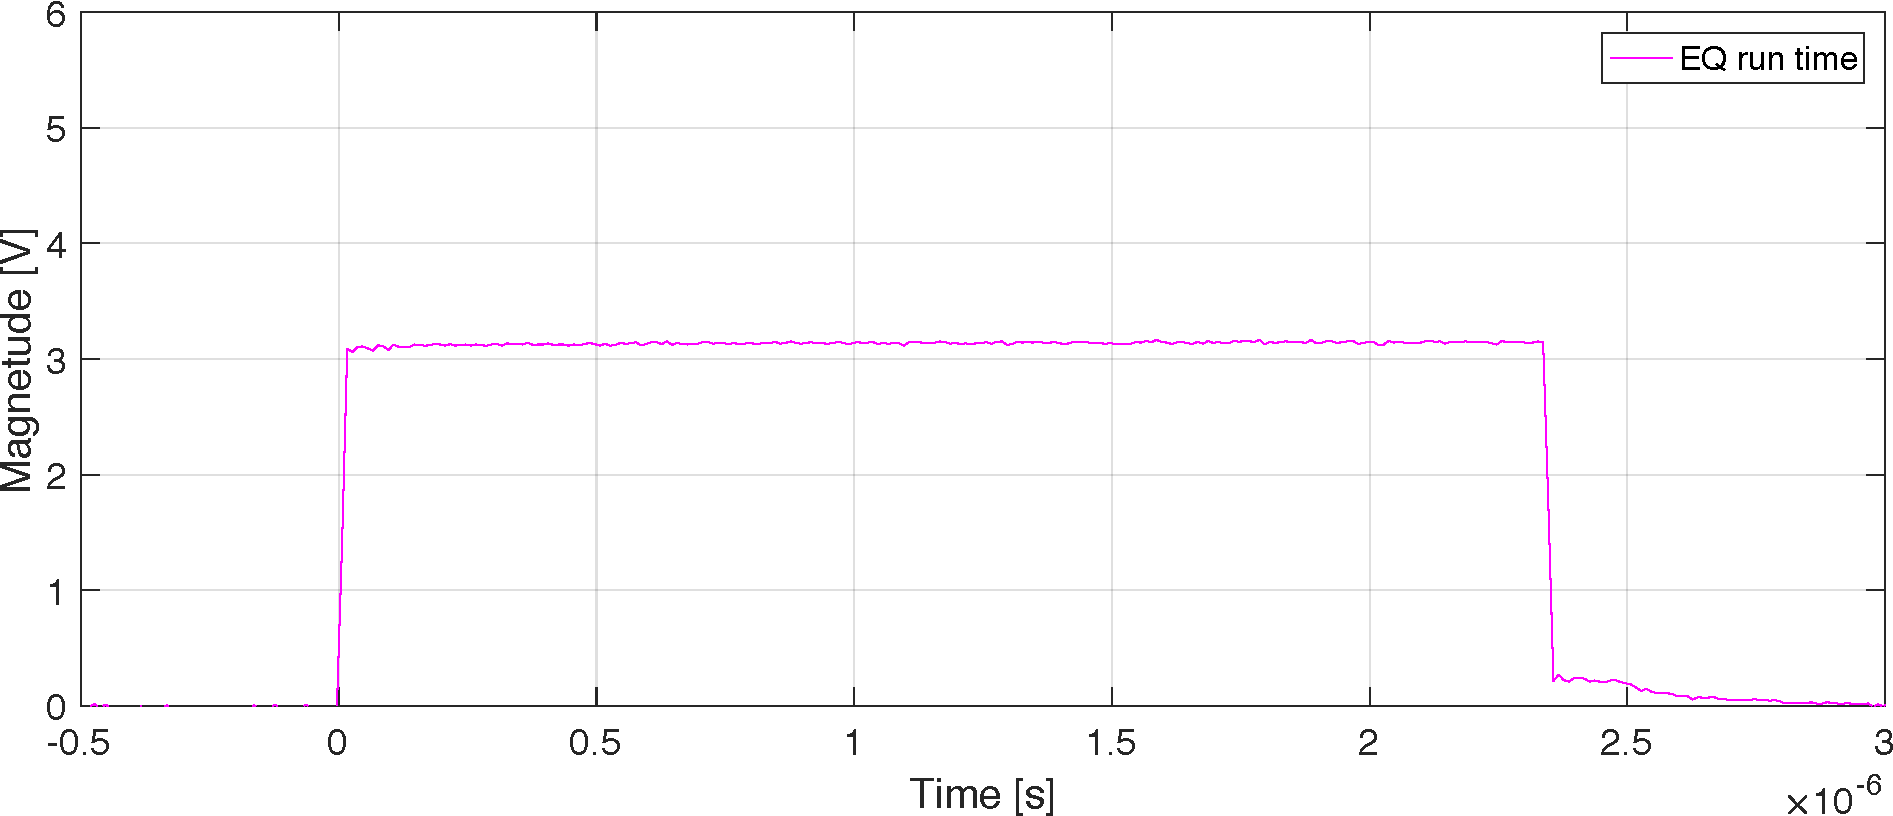
\includegraphics[width=1\textwidth]{eq_run_time.pdf}
		\caption{The figure shows the runtime of the flanger assembly program}
		\label{fig:eq_time_test}
\end{figure}

According to \autoref{fig:eq_time_test}, the equalizer run time is \SI{2.35}{\micro\second}.

\section*{Delay run time}
The following \autoref{fig:delay_time_test} shows the measurement results of the delay assembly program runtime.
\begin{figure}[htbp!]
	\centering
		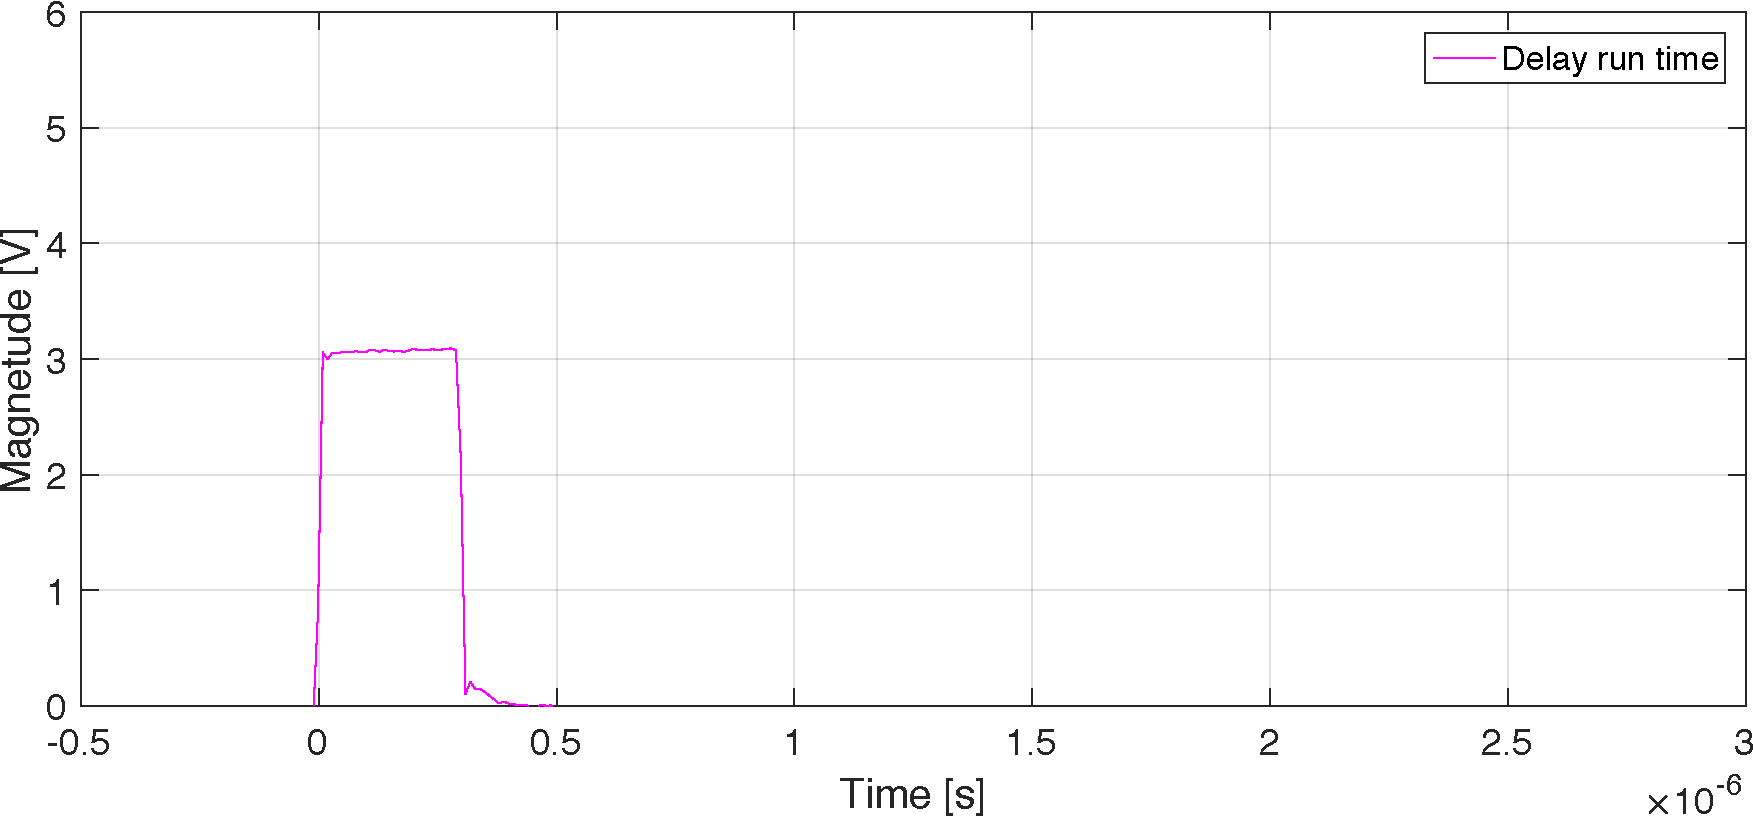
\includegraphics[width=1\textwidth]{delay_run_time.pdf}
		\caption{The figure shows the runtime of the delay assembly program}
		\label{fig:delay_time_test}
\end{figure}

According to \autoref{fig:delay_time_test}, the equalizer run time is \SI{300}{\nano\second}.